% =====================================================================
% WOWERS Master's Thesis — Tom's assembly file (Track T + Joint drafts)
% ---------------------------------------------------------------------
% This is the master LaTeX document. Tom drafts the data/backend chapters
% (Track T) and the Joint framing chapters here; Mohamed's frontend prose
% (M1, M2) drops into the marked [MERGE] stubs at combine time.
%
% WORKFLOW (see thesis/THESIS_BREAKDOWN.md):
%   - Write ONE work package at a time. Replace its \wptodo stub with prose.
%   - Obey thesis/thesis_format_prompt.md (voice, numbers, honesty, fig/tab rules).
%   - After a WP: tick it in THESIS_BREAKDOWN.md and log to thesis/THESIS_JOURNAL.md.
%
% COMPILE:  pdflatex thesis_tom.tex   (run twice for TOC/refs)
% =====================================================================
\documentclass[12pt,letterpaper]{report}

% Graduate-thesis page setup: 12pt double-spaced body, 1.5in binding margin.
\usepackage[left=1.5in,right=1in,top=1in,bottom=1in]{geometry}
\usepackage{setspace}
\doublespacing
\usepackage{graphicx}
\usepackage{booktabs}
\usepackage{amsmath}
\usepackage{caption}
\usepackage{etoolbox}
\usepackage{tocloft}

% Double spacing applies to body prose only. Captions, tabular bodies, and the
% reference list stay single-spaced, which is the usual thesis exemption.
\captionsetup{font=singlespacing}
\AtBeginEnvironment{tabular}{\singlespacing}
\AtBeginEnvironment{thebibliography}{\singlespacing\setlength{\itemsep}{0.6em}}
\usepackage[hidelinks]{hyperref}
\usepackage{xcolor}
\usepackage{tikz}
\usetikzlibrary{arrows.meta,positioning,fit,calc}

% --- format rule: figures and tables number sequentially across the WHOLE
% document (Figure 1, 2, 3 ... / Table 1, 2, 3 ...), not per chapter, and the
% appendix continues the same sequence rather than restarting.
\usepackage{chngcntr}
\counterwithout{figure}{chapter}
\counterwithout{table}{chapter}

% --- format rule §3.5: TOC / LoF / LoT render as dot-leader lines with page
% numbers. The report class gives leaders to sections but not to chapters.
\renewcommand{\cftchapleader}{\cftdotfill{\cftdotsep}}
\renewcommand{\cftchapfont}{\normalfont\bfseries}
\renewcommand{\cftchappagefont}{\normalfont\bfseries}

% --- helper: placeholder for a not-yet-written work package -----------
\newcommand{\wptodo}[2]{%
  \par\medskip\noindent\textcolor{red}{\textbf{[TODO — #1]}}\ \textit{#2}\par\medskip}

% --- helper: figure pending upload (per THESIS_BREAKDOWN images rule) ---
% Usage: \figpending{N}{what/where the image should come from}{caption text}
\newcommand{\figpending}[3]{%
  \begin{figure}[htbp]\centering
    \fbox{\parbox{0.85\linewidth}{\centering\vspace{1.5em}%
      \textbf{[FIGURE #1 PENDING --- awaiting upload: #2]}%
      \vspace{1.5em}}}
    \caption{#3}\label{fig:#1}
  \end{figure}}

% deprecated alias kept so older stubs still compile
\newcommand{\figplaceholder}[3]{\figpending{#1}{#2}{#3}}

\title{WOWERS: A Proof-of-Concept Infrastructure-Intelligence Platform for National
Screening of Micro-Hydropower Recovery at Wastewater Outfalls}
\author{XINSHENG (TOM) TANG \and MOHAMED ABDEL HAMID}
\date{} % set MONTH_YEAR on title page below

\begin{document}

% =====================================================================
% FRONT MATTER                                          (WP J5 — Joint)
% =====================================================================
\begin{titlepage}\centering
  {\large WOWERS: A Proof-of-Concept Infrastructure-Intelligence Platform for\\
   National Screening of Micro-Hydropower Recovery at Wastewater Outfalls\par}
  \vspace{2cm}
  A THESIS\\ SUBMITTED TO THE FACULTY OF THE GRADUATE SCHOOL\\
  OF UNIVERSITY OF ST.\ THOMAS\\ BY\par
  \vspace{1cm}
  XINSHENG (TOM) TANG\\ MOHAMED ABDEL HAMID\par
  \vspace{1cm}
  IN PARTIAL FULFILLMENT OF THE REQUIREMENTS\\
  FOR THE DEGREE OF MASTER OF SCIENCE\par
  \vspace{1cm}
  {\itshape \{\{MONTH\_YEAR\}\}}\par
\end{titlepage}

% Front matter is numbered in lowercase roman; the body restarts at arabic 1.
\pagenumbering{roman}

% --- Certification page ----------------------------------------------
\thispagestyle{empty}
\noindent UNIVERSITY OF ST.\ THOMAS\par\vspace{1em}
\noindent This is to certify that I have examined this copy of Master's thesis by\par
\vspace{1em}\noindent Xinsheng (Tom) Tang\\ Mohamed Abdel Hamid\par
\vspace{1em}\noindent and have found it is complete and satisfactory in all respects,
and that any and all revisions required by the final examining committee have been made.
\par\vspace{2em}
\noindent\rule{6cm}{0.4pt}\\ Name of Faculty Advisor(s)\par\vspace{1.5em}
\noindent\rule{8cm}{0.4pt}\\ Signature of Faculty Advisor(s)\par\vspace{1.5em}
\noindent\rule{8cm}{0.4pt}\\ Date\par\vspace{2em}
\noindent GRADUATE PROGRAM\\ School of Engineering\par
\clearpage

% --- Abstract (5 paragraphs, 350-450 words; write LAST) ---------------
\chapter*{Abstract}
\addcontentsline{toc}{chapter}{Abstract}
\wptodo{J5 · Abstract}{Five paragraphs per format §3.3: (1) opportunity + quantified loss;
(2) the proposal + "that can be built on later in the development of a minimum viable
product (MVP)"; (3) dataflow end to end; (4) headline numbers at full precision, measured
vs.\ simulated separated; (5) what it enables + three improvements. Write after all
chapters exist.}

% --- Acknowledgements -------------------------------------------------
\chapter*{Acknowledgements}
\addcontentsline{toc}{chapter}{Acknowledgements}
\wptodo{J5 · Acknowledgements}{Four short paragraphs: advisor; business-side faculty;
named industry practitioners; one-line catch-all.}

% tocloft does not force a page break before each list, so the \clearpage calls
% below are required — without them Contents runs on from Acknowledgements.
\begin{singlespace}
\clearpage
\tableofcontents
\clearpage
\addcontentsline{toc}{chapter}{List of Figures}
\listoffigures
\clearpage
\addcontentsline{toc}{chapter}{List of Tables}
\listoftables
\end{singlespace}
\clearpage

% Body pages restart at arabic 1 per standard graduate-thesis pagination.
\pagenumbering{arabic}

% =====================================================================
% CHAPTER 1 — INTRODUCTION                              (WP J2 — Joint)
% =====================================================================
\chapter{Introduction}
\wptodo{J2 · Introduction (~1,100 w)}{Macro trend + hard number; why current approach does
not scale; "We propose the creation of a company, WOWERS, to\dots"; end-state workflow;
split technical vs.\ logistical development. Feeds: ARCHITECTURE.md, project journal.}

\section{Thesis Statement}
\wptodo{J2}{One paragraph ~120 words: the proposition, scope of the business discussion,
what the proof-of-concept develops.}

\section{Thesis Outline}
\wptodo{J2}{One paragraph walking each chapter in order.}

% =====================================================================
% CHAPTER 2 — BACKGROUND AND PRIOR WORK                 (WP T1 — Tom)
% =====================================================================
\chapter{Background and Prior Work}

Municipal wastewater treatment is an energy-intensive public service. Nationally,
U.S.\ publicly owned treatment works (POTWs) consume on the order of 30.2 TWh/yr of
electricity, about 0.8\% of total U.S.\ electricity use in the reference year of the
Electric Power Research Institute (EPRI) sector study~\cite{epri2013}. At the same time,
treated effluent leaves most plants through gravity or pressurized outfalls that drop
several meters of unused hydraulic head into receiving waters. That residual head is
dissipated as turbulence and heat rather than converted to useful work. Micro-hydropower
recovery at the outfall is therefore an energy-\emph{recovery} opportunity nested inside
an energy-\emph{consuming} facility: the plant already pays for aeration, pumping, and
solids handling, while a fraction of the kinetic and potential energy in the discharge
stream goes unused.

The physical opportunity is real, but capture has been rare. There are six common
limitations that keep outfall energy recovery from scaling across the U.S.\ POTW fleet.
These limitations will now be discussed in more detail.

\section{Wastewater Outfall Energy Loss and Recovery Limitations}

The six limitations that dominate practice are (1)~unmeasured site head, (2)~incomplete
or corrupted flow records, (3)~misapplied river-hydro capacity factors, (4)~debris and
maintenance downtime that physics models omit, (5)~project-by-project rather than
fleet-scale screening, and (6)~opaque unit economics relative to plant power bills.
Each limitation is treated below in that order.

Unmeasured hydraulic head is the first barrier. Gross head at an outfall is the elevation
difference between the plant hydraulic grade line and the receiving-water surface, less
friction and minor losses in the conduit. Unlike river dams, WWTP outfalls are not
instrumented with published stage records, and national permit databases carry facility
coordinates far more reliably than outfall invert elevations. Screening studies that
substitute literature archetype heads (for example triangular distributions of a few
meters for small plants) can mis-rank sites by a factor of two or more when real
topographic relief differs from the archetype~\cite{ornl2014}. Rule of thumb in the field
is that net heads below about 1--2~m rarely justify a conventional reaction turbine
without a very large continuous flow.

Incomplete or corrupted discharge records form the second barrier. Flow is reported to
EPA through Discharge Monitoring Reports (DMRs) under ICIS-NPDES, but the national archive
contains sentinel values (for example design-flow entries of 999.0~MGD), unit slips between
gallons per day and million gallons per day, and primary-outfall selection errors that
prefer a single corrupted row over a consistently reported treatment outfall. After
cleaning, the WOWERS Phase~1 cohort retains 17,148 active POTWs with usable mean flow; the
pre-clean archive required extensive guards precisely because uncorrected DMR rows
propagate into energy estimates that look precise and are wrong~\cite{epa_echo}.

Capacity-factor misapplication is the third barrier. Run-of-river small hydro in the DOE
HydroSource Existing Hydropower Assets (EHA) dataset shows median annual capacity factors
near 0.39 for plants in the 0.1--5~MW class (629 plants, 9,798 plant-years) because of
seasonal drought, peak sizing, and environmental-flow bypasses~\cite{hydrosource_eha}.
WWTP outfalls track municipal demand, typically varying only $\pm$15--25\% seasonally, and
have no ecological minimum-flow reservation on the effluent itself. Applying the river
median CF to a continuous municipal conduit therefore understates recoverable energy by
roughly a factor of two relative to a WWTP-appropriate CF near 0.60, the central
tier we adopt after anchoring to LucidPipe~\cite{lucidpipe}.

Debris fouling, minimum-flow cutoffs, and maintenance downtime constitute the fourth
limitation. Physics ceilings that integrate $\eta\rho g Q H$ over a flow-duration curve
with high availability (implied CF near 0.87 in the WOWERS Phase~2 P50 ceiling of
409.2~GWh/yr) omit screens clogging, grit abrasion in wastewater, and planned outages.
Even the best-documented continuous-conduit anchor---LucidPipe Portland at measured CF
0.628---already sits well below a pure physics ceiling~\cite{lucidpipe}. Expecting
fleet-wide CF above about 0.65 without site-specific O\&M modeling is not supported by
published installs.

The fifth limitation is institutional rather than hydraulic: recovery projects are
originated one municipality at a time. Vendors such as LucidEnergy, Rentricity, and CINK
Hydro-Energy publish case sheets for individual pressurized mains or WWTP references, but
no public national inventory ranks all U.S.\ POTW outfalls by recoverable energy and
payback under a shared method~\cite{rentricity,cink}. Without a fleet screen, capital
flows to the plants that already have a consultant, not necessarily to the plants with the
best physics.

The sixth limitation is economic opacity at plant scale. EPRI reports national wastewater
electricity use of 30.2~TWh/yr and observed energy intensities from about 3,300~kWh/MG for
plants under 2~MGD down to about 1,600~kWh/MG for plants above 100~MGD~\cite{epri2013}.
Against that bill, a micro-turbine that offsets a median of roughly 0.8\% of plant
consumption (Phase~4 screening sanity check) looks trivial in isolation even when the
portfolio NPV is large. Operators therefore under-invest unless screening shows named
payback, CapEx, and turbine match rather than a generic ``green energy'' claim.
These common limitations will now be set against what current practice already achieves.

\section{Current Practice and In-Conduit Recovery Techniques}

In-conduit and effluent hydropower is a proven niche, not an empty category. Three
commercial lines illustrate what practitioners already do well, which of the six
limitations they address, and which they leave open.

LucidEnergy's LucidPipe system places spherical in-pipe turbines in large-diameter
pressurized transmission mains (approximately 24--96~in). The flagship Portland, Oregon,
installation on the Bull Run drinking-water main deploys four 42~in machines for 200~kW
nameplate capacity and reports 1,100~MWh/yr of generation, implying a measured capacity
factor of $1{,}100{,}000/(200\times 8{,}760)=0.628$~\cite{lucidpipe}. That project
demonstrates continuous municipal-conduit duty cycles with CF well above river-hydro
medians, and it catches limitation~(3) by proving the WWTP/conduit CF argument in the
field. It does not catch limitations~(1),~(5), or~(6) for the national WWTP fleet: head and
flow are known because the utility already operates the main, and the project was
originated as a single utility partnership rather than from a ranked national list. The
hydraulic regime is also drinking water rather than wastewater, so debris and corrosion
risks are milder than at a secondary-effluent outfall.

Rentricity supplies reverse-pump (Francis-type) machines certified to NSF~61/372 for
potable and wastewater service. Public featured projects include approximately 32~kW at
2.4~MGD and 40~psi, and approximately 360~kW at 2--12~MGD with 175--250~ft of head
~\cite{rentricity}. These installs show that wastewater-certified hardware exists in the
tens-to-hundreds-of-kilowatts band relevant to medium POTWs, addressing part of
limitation~(4) through productized O\&M expectations. Annual generation (hence CF) is not
published per site, so Rentricity cannot yet anchor a national calibration band the way
LucidPipe can. Screening still depends on the utility bringing a known pressure and flow
to the vendor.

CINK Hydro-Energy manufactures crossflow, Kaplan, Pelton, and Francis machines and
explicitly lists wastewater treatment plants among use cases. The company reports more than
450 turbines in more than 50 countries and advertises operation from 6\% to 100\% of design
flow~\cite{cink}. That part-load envelope is well matched to flat municipal flow-duration
curves and therefore softens limitation~(4) relative to peak-sized river machines. As with
Rentricity, published per-site annual kWh figures suitable for CF calibration are sparse,
and project origination remains site-solicited rather than fleet-ranked.

Complementary U.S.\ vendors (Canyon Hydro conduit installations, Emrgy canal modules,
Turbulent vortex units, Natel fish-safe Kaplan variants) enlarge the hardware menu but do
not change the pattern: hardware and site engineering exist; a reproducible national
prioritization of POTW outfalls does not~\cite{doe_vision}. Current practice therefore
catches local hydraulic feasibility and, in the LucidPipe case, continuous-conduit CF. It
misses national ranking under shared assumptions, systematic treatment of DMR data quality,
and calibrated portfolio energy bands. A public-data screening primer that makes those
gaps precise will now be discussed.

\section{Public-Data Screening of Hydropower Potential (Primer)}

This section discusses only the \emph{screening} problem---estimating which plants merit
a site visit---not detailed civil design, interconnection studies, or turbine manufacturing.
The enabling physics is the standard hydropower relation
\begin{equation}
  P = \eta\,\rho\,g\,Q\,H,
  \label{eq:hydro}
\end{equation}
where $P$ is electrical power, $\eta$ is overall efficiency, $\rho$ is water density,
$g$ is gravitational acceleration, $Q$ is volumetric flow, and $H$ is net head. Annual
energy follows by integrating power over time, or equivalently by integrating
Equation~\eqref{eq:hydro} along a flow-duration curve (FDC) with an availability factor.
For municipal outfalls, $Q$ is observed (DMR monthly averages), while $H$ must be inferred
from topography or plant drawings.

Three public data layers make a national screen possible in principle. First, EPA ECHO /
ICIS-NPDES identifies active POTW permits and publishes facility attributes used to build
the candidate set~\cite{epa_echo}. Second, DMR parameter 50050 (flow) supplies the time
series from which mean flow, percentiles, and a 20-point FDC are computed; the WOWERS
ingest processes on the order of 279~million DMR rows spanning fiscal years 2009--2024.
Third, the USGS 3DEP elevation service supplies point elevations that, differenced between
plant and outfall coordinates and reduced by a head-loss fraction, yield a DEM-proxy net
head in place of literature archetype triangles~\cite{usgs_3dep}. Ground-truth generation
and capacity-factor benchmarks additionally draw on EIA/EHA HydroSource tables for existing
hydropower assets~\cite{hydrosource_eha}.

A defensible screen must still separate physics ceilings from calibrated expectations.
Substituting median river-hydro CF for continuous effluent over-haircuts energy; omitting
debris and downtime overstates it. The WOWERS response, developed in Chapters~4 and~5, is
to report a physics ceiling (409.2~GWh/yr at the P2-SEED baseline) beside a calibrated band
of 119--281~GWh/yr anchored to EHA empirics and LucidPipe~\cite{hydrosource_eha,lucidpipe}. Prior national
methods that stop at resource potential, or that calibrate only against river fleets,
therefore leave a methodological gap that Section~2.4 compares explicitly. Why those prior
methods remain limited for POTW outfall recovery will now be discussed.

\section{Prior National Assessments and Calibration Approaches}

National hydropower assessment literature is rich for rivers and canals and thin for
WWTP outfalls. The comparison that follows uses a single common metric---reported or
implied annual energy (or capacity factor) at national or multi-state scale---across at
least three named prior lines of work and the WOWERS screen. The scale and method contrast
can be seen in Table~\ref{tab:prior_work}.

\begin{table}[htbp]
  \centering
  \caption{Comparison of national and conduit hydropower assessment approaches by scope,
  primary flow/head basis, and headline energy or capacity-factor metric}
  \label{tab:prior_work}
  \begin{tabular}{@{}p{2.6cm}p{2.8cm}p{3.2cm}p{3.6cm}@{}}
    \toprule
    Assessment & Scope & Flow / head basis & Headline metric \\
    \midrule
    DOE Hydropower Vision (2016) & U.S.\ conventional + new stream-reach & Resource + cost
      curves; not POTW-specific & Sector roadmap; small-hydro cost form
      $A\cdot\mathrm{kW}^{B}$~\cite{doe_vision,ornl2014} \\
    ORNL / HydroSource EHA CF & Existing U.S.\ plants $\geq$1~MW class tabulated & Metered
      generation / nameplate & Median CF $\approx$0.39 (0.1--5~MW bucket,
      629 plants)~\cite{hydrosource_eha} \\
    ORNL conduit / BCM canal methods & Non-powered dams, canals, municipal conduit cost
      samples & Engineering potential + install-cost equations & Potential GWh and
      \$/kW fits (e.g.\ BCM ICC)~\cite{ornl2014,osti3002705} \\
    WOWERS (this work) & 17,148 U.S.\ POTW outfalls $\rightarrow$ 1,138 project-viable &
      ICIS DMR FDC + 3DEP head proxy; CF calibrated & Physics ceiling 409.2~GWh/yr;
      calibrated band 119--281~GWh/yr \\
    \bottomrule
  \end{tabular}
\end{table}

DOE's \emph{Hydropower Vision} and the related Oak Ridge National Laboratory (ORNL) New
Stream-reach Development cost work supply the sector framing and the power-law CapEx form
used throughout small-hydro screening, but they do not inventory WWTP effluent
drops~\cite{doe_vision,ornl2014}. Their value to WOWERS is methodological (cost curves,
turbine envelopes), not a POTW energy total that can be compared one-to-one with
409.2~GWh/yr.

The HydroSource EHA annual capacity-factor workbook is the strongest empirical
calibration source available without site visits. Restricting to the 0.1--5~MW class yields
629 plants and 9,798 plant-years with median CF 0.390 and 25th/75th percentiles 0.254 /
0.541~\cite{hydrosource_eha}. Those statistics correctly bound a \emph{conservative
floor} for any small-hydro claim. They incorrectly describe WWTP duty cycles if used as a
central estimate, because seasonal river drivers listed in Section~2.1 do not apply to
municipal effluent. The WOWERS calibration therefore keeps the EHA floor (119--194~GWh/yr
depending on percentile and MW sub-bucket) and adds a WWTP-appropriate central tier at
CF~0.60 (281~GWh/yr) anchored 5\% below LucidPipe's measured 0.628~\cite{lucidpipe}.

ORNL conduit and canal work, including municipal conduit install-cost samples and the
baseload cost model (BCM) canal/conduit installed-capital-cost equation, improves CapEx
realism for in-conduit machines but again estimates \emph{engineering potential} or
\$/kW rather than a cleaned national POTW energy band tied to DMR
FDCs~\cite{ornl2014,osti3002705}. FERC's qualifying-conduit pathway under the Hydropower
Regulatory Efficiency Act of 2013 further lowers soft costs for man-made municipal conduits
(Notice of Intent rather than a full license for facilities $\leq$40~MW), which improves
project economics once a site is chosen but does not rank sites~\cite{ferc_conduit}.

Plant energy-\emph{consumption} literature (EPRI Table~5-1 observed kWh/MG by flow band;
WEF Manual of Practice~32 curves retained for sensitivity) closes the offset narrative:
national wastewater use near 30.2~TWh/yr and validated plant-level intensities give context
for why a 119--281~GWh/yr recovery band is simultaneously material at portfolio scale and
small as a fraction of treatment load~\cite{epri2013,wef_mop32}. ENERGY STAR and EPA
planning guides corroborate the order of magnitude without replacing the EPRI observed
grid~\cite{epa2013}.

Taken together, prior assessments either (a)~quantify broad hydropower resource and cost,
(b)~measure CF on river fleets, or (c)~document individual conduit installs. None combine a
17,000-plant POTW filter, DMR-derived FDCs, DEM-proxy heads, vendor turbine matching, and
an explicit physics-versus-calibrated energy band. That combined screen is the technical
core developed in Chapter~4, and the quantitative gaps between ceiling and calibrated
expectation are reported in Chapter~5. The business model that motivates building such a
screen will now be discussed.

% =====================================================================
% CHAPTER 3 — BUSINESS MODEL                            (WP J1 — Joint)
% =====================================================================
\chapter{Business Model}
\wptodo{J1 · Ch3 (~2,300 w)}{Eight subsections, 150--400 w each. Feeds:
WOWERS\_Project\_Report.pdf, DIRECTOR\_BRIEF\_2026-06-24.md,
WOWERS\_Capital\_and\_Funding\_Research.md, Fowler feedback. Address the four judge gaps.}

\section{The Problem}
\wptodo{J1 · 3.1}{Global/national \$ figure + unit-level figure + three named complications.}
\section{The Solution}
\wptodo{J1 · 3.2}{The service in one paragraph; optional partner/ecosystem play.}
\section{The Target Market}
\wptodo{J1 · 3.3}{One REAL named archetype plant: size, output, what makes it hard to serve.}
\section{Competition}
\wptodo{J1 · 3.4}{Real competitors (LucidEnergy, Rentricity, CINK); concede strengths; the gap.}
\section{Pricing Model}
\wptodo{J1 · 3.5}{Three price tiers (bulleted, \$ figures) + one derivation sentence.}
\section{Marketing and Distribution}
\wptodo{J1 · 3.6}{Three named stages, in order, goal of each.}
\section{Market Potential}
\wptodo{J1 · 3.7}{TAM$\rightarrow$SAM$\rightarrow$SOM arithmetic shown; ~10\% realistic share.}
\section{Future Vision and Project Timeline}
\wptodo{J1 · 3.8}{Named upcoming project; milestone sequence; which milestone is built first.}

% =====================================================================
% CHAPTER 4 — DESIGN DETAILS (technical bulk, 9,000-12,000 w)
% Hardware skeleton remapped to WOWERS software (see BREAKDOWN §0).
% =====================================================================
\chapter{Design Details}

\section{System Overview}                                % WP T2 / Joint

The WOWERS platform is a national screening system that turns public regulatory
and geospatial data into ranked, financially scored micro-hydropower opportunities
at U.S.\ POTW outfalls. Figure~\ref{fig:1} below depicts the top-level dataflow.
Four external source families feed a four-phase Python pipeline; the pipeline
writes parquet intermediates; an export script freezes a 58-property GeoJSON
contract; and a React + MapLibre dashboard reads that single file with no live
backend.

\begin{figure}[htbp]
  \centering
  % Self-contained TikZ — compiles on Overleaf with no external PNG upload.
  \resizebox{\textwidth}{!}{%
  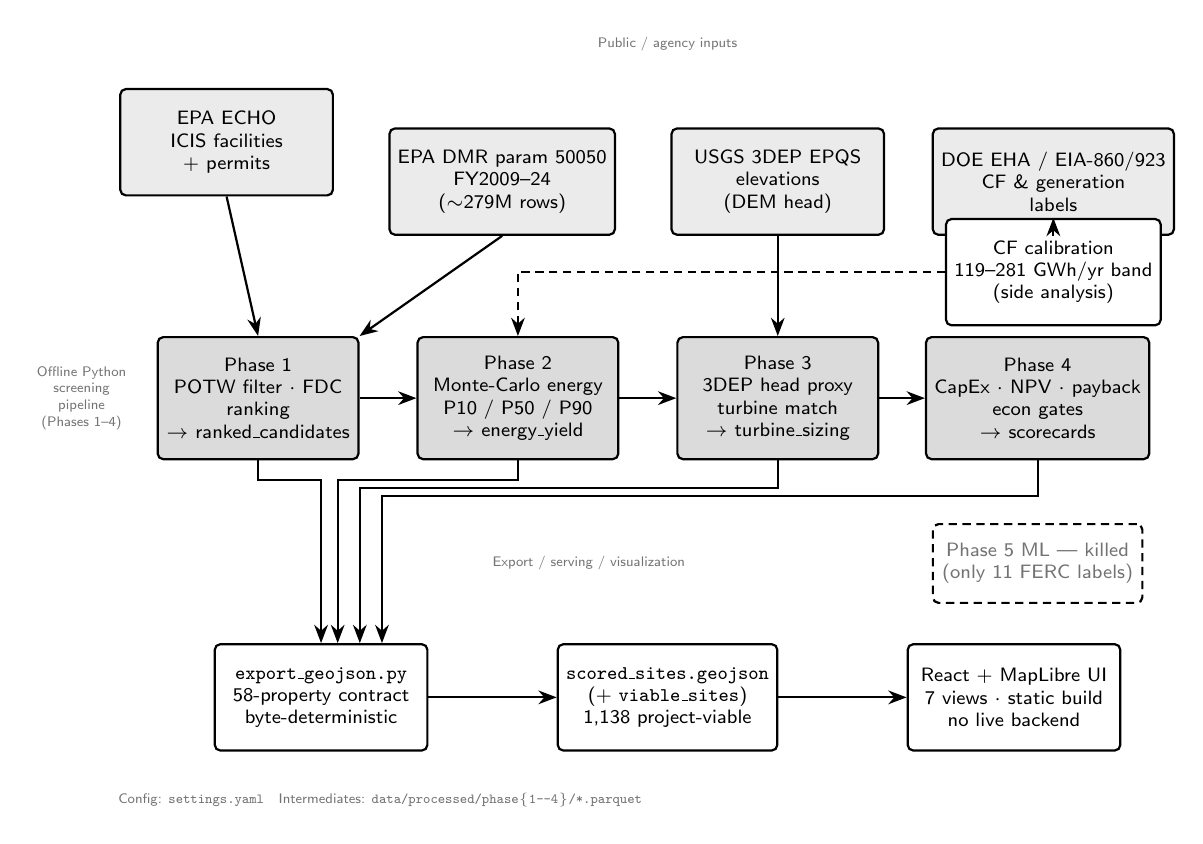
\begin{tikzpicture}[
    font=\sffamily\scriptsize,
    >=Stealth,
    every node/.style={align=center},
    src/.style={draw, thick, rounded corners=2pt, fill=black!8,
      minimum width=2.7cm, minimum height=1.35cm, inner sep=3pt},
    phase/.style={draw, thick, rounded corners=2pt, fill=black!14,
      minimum width=2.55cm, minimum height=1.55cm, inner sep=3pt},
    art/.style={draw, thick, rounded corners=2pt, fill=white,
      minimum width=2.7cm, minimum height=1.35cm, inner sep=3pt},
    kill/.style={draw, thick, densely dashed, rounded corners=2pt,
      fill=white, text=black!55, minimum width=2.55cm, minimum height=1.0cm},
    lbl/.style={font=\sffamily\tiny, text=black!55},
    arr/.style={->, thick},
  ]
    % --- labels ---
    \node[lbl] at (5.6, 6.05) {Public / agency inputs};
    \node[lbl, anchor=east] at (-1.15, 1.55) {Offline Python\\screening\\pipeline\\(Phases 1--4)};
    \node[lbl] at (4.6, -0.55) {Export / serving / visualization};

    % --- sources ---
    \node[src] (echo) at (0.0,4.8) {EPA ECHO\\ICIS facilities\\+ permits};
    \node[src] (dmr)  at (3.5,4.3) {EPA DMR param 50050\\FY2009--24\\($\sim$279M rows)};
    \node[src] (dep)  at (7.0,4.3) {USGS 3DEP EPQS\\elevations\\(DEM head)};
    \node[src] (eha)  at (10.5,4.3) {DOE EHA / EIA-860/923\\CF \& generation\\labels};

    % --- phases ---
    \node[phase] (p1) at (0.4,1.55) {Phase 1\\POTW filter $\cdot$ FDC\\ranking\\$\rightarrow$ ranked\_candidates};
    \node[phase] (p2) at (3.7,1.55) {Phase 2\\Monte-Carlo energy\\P10 / P50 / P90\\$\rightarrow$ energy\_yield};
    \node[phase] (p3) at (7.0,1.55) {Phase 3\\3DEP head proxy\\turbine match\\$\rightarrow$ turbine\_sizing};
    \node[phase] (p4) at (10.3,1.55) {Phase 4\\CapEx $\cdot$ NPV $\cdot$ payback\\econ gates\\$\rightarrow$ scorecards};

    % --- CF side analysis + Phase 5 kill ---
    \node[art] (cf) at (10.5,3.15) {CF calibration\\119--281 GWh/yr band\\(side analysis)};
    \node[kill] (p5) at (10.3,-0.55) {Phase 5 ML --- killed\\(only 11 FERC labels)};

    % --- export row ---
    \node[art] (exp) at (1.2,-2.25) {\texttt{export\_geojson.py}\\58-property contract\\byte-deterministic};
    \node[art] (gj)  at (5.6,-2.25) {\texttt{scored\_sites.geojson}\\(+ \texttt{viable\_sites})\\1,138 project-viable};
    \node[art] (ui)  at (10.0,-2.25) {React + MapLibre UI\\7 views $\cdot$ static build\\no live backend};

    % --- arrows: sources -> phases ---
    \draw[arr] (echo.south) -- (p1.north);
    \draw[arr] (dmr.south)  -- (p1.north east);
    \draw[arr] (dep.south)  -- (p3.north);
    \draw[arr] (eha.south)  -- (cf.north);
    \draw[arr, densely dashed] (cf.west) -| (p2.north);

    % --- phase chain ---
    \draw[arr] (p1) -- (p2);
    \draw[arr] (p2) -- (p3);
    \draw[arr] (p3) -- (p4);

    % --- phases fan into export ---
    \draw[arr] (p1.south) -- ++(0,-0.25) -| (exp.north);
    \draw[arr] (p2.south) -- ++(0,-0.25) -| ([xshift=6pt]exp.north);
    \draw[arr] (p3.south) -- ++(0,-0.35) -| ([xshift=14pt]exp.north);
    \draw[arr] (p4.south) -- ++(0,-0.45) -| ([xshift=22pt]exp.north);

    % --- export chain ---
    \draw[arr] (exp) -- (gj);
    \draw[arr] (gj) -- (ui);

    \node[lbl, anchor=west] at (-1.5,-3.55)
      {Config: \texttt{settings.yaml}\quad
       Intermediates: \texttt{data/processed/phase\{1--4\}/*.parquet}};
  \end{tikzpicture}%
  }
  \caption{System block diagram of the WOWERS platform}
  \label{fig:1}
\end{figure}

Data enter as EPA ECHO / ICIS-NPDES facility and permit tables, approximately
279~million Discharge Monitoring Report (DMR) rows for fiscal years 2009--2024,
USGS 3DEP elevation point queries, and DOE HydroSource Existing Hydropower Assets
(EHA) / EIA Form~860--923 tables used for capacity-factor calibration and the
attempted Phase~5 ground-truth set. Phase~1 filters active POTWs, builds monthly
flow series, computes flow features, and ranks candidates. Phase~2 runs a
site-keyed Monte-Carlo energy engine that produces P10/P50/P90 annual energy under
Equation~\eqref{eq:hydro}. Phase~3 replaces literature head archetypes with a
3DEP DEM proxy where coordinates allow, then matches commercial turbine envelopes.
Phase~4 applies CapEx/OpEx models, revenue and plant-consumption offsets, and
NPV/IRR/payback gates that define the project-viable cohort. The P2-SEED re-baseline
that Chapter~5 reports screens 17,148 POTWs and retains 1,138 project-viable sites
with a physics ceiling of 409.2~GWh/yr, a calibrated band of 119--281~GWh/yr,
portfolio NPV of \$310.1M, and median payback of 9.8~yr.

Configuration is centralized in \texttt{config/settings.yaml} (URLs, fiscal-year
list, sanity caps, ranking weights, physics constants, cost-model coefficients).
Ingest and transforms are implemented in \texttt{polars} with chunked DMR reads
(\texttt{processing.dmr\_chunk\_size} $= 500{,}000$) and parquet checkpoints under
\texttt{data/processed/phase\{1--4\}/}. The serving boundary is deliberate: the
dashboard consumes only \texttt{exports/viable\_sites.geojson} (and the companion
scored-sites file), so pipeline and UI can evolve on opposite sides of a frozen
property contract.

For this work, although a full screening solution has been implemented, it does
not strictly follow the originally proposed design and functions as a proof of
concept. The notable differences in design are (1)~head is a DEM proxy with a
plausibility gate rather than surveyed invert elevations or plant drawings;
(2)~Phase~5 supervised learning was killed after only eleven FERC conduit labels
were found, so no ML energy model ships; (3)~the dashboard is a static Vite build
over a single GeoJSON file rather than a live API over parquet; and (4)~revenue
and CapEx remain modeled bands (power-law \$/kW, EPRI kWh/MG intensities, FERC
conduit NOI assumptions) rather than vendor quotes or metered plant bills. Those
gaps are intentional for a national screen and are named again in the subsystem
sections that follow. How the raw data that drive this pipeline are acquired will
now be discussed.

\section{Data Acquisition}                               % WP T2 — Tom

Data acquisition is responsible for placing every external input the pipeline
needs onto local disk in a form later phases can read without re-hitting vendor
portals on every run. There are four main requirements of acquisition. The
ingest must (1)~cover the national POTW fleet rather than a convenience sample,
(2)~preserve enough multi-year flow history to build an FDC, (3)~supply
coordinates accurate enough for a 3DEP head proxy, and (4)~admit an independent
capacity-factor or generation label set for calibration. The source inventory
satisfying those requirements can be seen in Table~\ref{tab:data_sources}.

\begin{table}[htbp]
  \centering
  \caption{Data-source inventory for the WOWERS screening pipeline}
  \label{tab:data_sources}
  \begin{tabular}{@{}p{2.4cm}p{3.4cm}p{2.6cm}p{3.4cm}@{}}
    \toprule
    Source & What it supplies & Approx.\ volume & Ingest module \\
    \midrule
    EPA ECHO ICIS facilities + permits
      & POTW identity, design/avg flow, permit status, facility lat/lon
      & \texttt{npdes\_downloads.zip} $\sim$322~MB
      & \texttt{src/phase1/ingest.py}, \texttt{filter\_potw.py} \\
    EPA ECHO DMR FY2009--24
      & Monthly flow (param 50050) by outfall
      & $\sim$279M rows; $\sim$9.6~GB ZIPs
      & \texttt{dmr\_timeseries.py} \\
    USGS 3DEP EPQS
      & Point elevation (m ASL) at plant/outfall coords
      & On-demand JSON; disk-cached
      & \texttt{src/phase3/elevation.py} \\
    DOE HydroSource EHA + EIA-860/923
      & Existing-hydro CF, net generation, nameplate
      & Plant + CF workbooks on disk
      & \texttt{src/phase5/ground\_truth.py}; \texttt{scripts/cf\_calibration.py} \\
    \bottomrule
  \end{tabular}
\end{table}

\subsection{Facility and Permit Tables (EPA ECHO / ICIS-NPDES)}

Three options were considered for the facility universe: (A)~manual municipal
outreach and FOIA per utility, (B)~Clean Watersheds Needs Survey (CWNS) plant
lists without NPDES join keys, and (C)~EPA ECHO bulk ICIS downloads. Option~(A)
cannot reach 17,000 plants in a thesis timeline. Option~(B) lacks the permit and
DMR join path required for measured flow. Option~(C) won because
\texttt{https://echo.epa.gov/files/echodownloads/npdes\_downloads.zip} already
bundles \texttt{ICIS\_FACILITIES.CSV} and \texttt{ICIS\_PERMITS.CSV} with a
stable join key (\texttt{NPDES\_ID} $=$ \texttt{EXTERNAL\_PERMIT\_NMBR}) and is
refreshable without vendor contracts~\cite{epa_echo}.

Implementation lives in \texttt{ingest\_npdes\_facilities} and
\texttt{load\_potw\_facilities}. The ZIP is streamed with retries, extracted once,
and skipped on re-run when the on-disk size matches. Permits are filtered to POTW
facility-type indicators, active status codes (including Administratively Continued
\texttt{ADC}, which recovered 4,308 permits including DC0021199 Blue Plains), and
non-federal treatment plants. Design and actual-average flow fields are scrubbed
before join: values above 2,000~MGD, the EPA numeric sentinel 999.0, and entries
below 0.005~MGD are nulled in \texttt{filter\_potw.py} so they cannot win a
``largest design flow'' deduplication. After the facilities join, P1-COORD-GUARD
drops rows whose latitude/longitude fall outside inclusive U.S.\ NPDES territory
bands (American Samoa, Guam/CNMI, CONUS--Alaska, USVI), rejecting rather than
auto-flipping obvious sign errors so hidden coordinate edits never enter the
parquet. The limitation deferred to future work is outfall-invert elevation: ICIS
gives facility geocodes, not surveyed hydraulic grade lines.

\subsection{Discharge Monitoring Reports (Flow Time Series)}

Three options were considered for flow: (A)~design flow only from the permit table,
(B)~utility SCADA exports, and (C)~national DMR parameter 50050. Design flow alone
cannot support an FDC or capacity-factor story. SCADA does not exist as a public
national archive. DMR won as the only measured monthly flow series covering
essentially the full permitted fleet. Fiscal years 2009--2024 are configured in
\texttt{settings.yaml} under \texttt{epa.dmr\_fiscal\_years}; each year downloads
from \texttt{npdes\_dmrs\_fy\{year\}.zip} with up to four parallel workers in
\texttt{ingest\_dmr\_files}.

Parsing in \texttt{dmr\_timeseries.py} reads each CSV in 500{,}000-row chunks with
\texttt{polars}, keeps parameter code \texttt{50050}, and resolves column-name
aliases that drift across fiscal years. The critical value rule is to prefer
\texttt{DMR\_VALUE\_STANDARD\_UNITS} (EPA-converted MGD) and fall back to
\texttt{DMR\_VALUE\_NMBR} only when the standard-units column is absent; using the
raw number as MGD when facilities report gal/d inflates flow by roughly
$10^{5}$ and was observed to push national means into the thousands of MGD before
the fix. NODI codes map selected ``no data'' indicators to zero or estimated
flags; other NODI values become null. Per-record caps at
$\max(2~\mathrm{MGD},\,10\times\mathrm{design\_flow})$ null corrupt rows before
feature statistics so a single 7{,}000~MGD typo cannot dominate a 0.02~MGD plant.
Primary-outfall selection prefers the outfall with the most non-null months rather
than the maximum mean, which previously let a rarely reported CSO/STR feature beat
the treatment outfall. The named limitation is residual \texttt{dmr\_limited}
sites with fewer than three surviving months: they are excluded or flagged before
Monte Carlo rather than imputed into false precision.

\subsection{Elevation (USGS 3DEP) and Calibration Labels (EHA / EIA)}

Head acquisition compared (A)~literature triangular archetypes only, (B)~paid DEM
tiles processed offline, and (C)~USGS Elevation Point Query Service (EPQS) v1
against plant and outfall coordinates. Archetypes alone are the Phase~2 bootstrap
but were already identified in Chapter~2 as a ranking risk. Offline tiles add
licensing and batch GIS overhead without improving the first national pass.
EPQS won for rebuildability: \texttt{src/phase3/elevation.py} queries
\texttt{https://epqs.nationalmap.gov/v1/json} with \texttt{httpx}/\texttt{asyncio},
honours \texttt{phase3.max\_concurrent\_requests} and \texttt{request\_delay\_s},
caches JSON under \texttt{data/elevation\_cache/} keyed by rounded lat/lon, and
treats the EPQS ocean sentinel $-1{,}000{,}000$ as a failed query~\cite{usgs_3dep}.
Outfall coordinates, when present in
\texttt{NPDES\_PERM\_FEATURE\_COORDS.csv}, enable a plant-minus-outfall DEM proxy;
otherwise the pipeline falls back through literature head then a design default.
The largest methodological assumption in the entire acquisition chain---that DEM
differencing approximates net hydraulic head---is deferred in detail to
Section~4.3.4.

Calibration and ground-truth acquisition compared (A)~no empirical CF check,
(B)~vendor case sheets only, and (C)~DOE HydroSource EHA annual capacity-factor
tables plus EIA-860/923 conventional-hydro generation. Option~(C) won for the
floor and central band reported in Chapter~2: EHA supplies 629 plants /
9{,}798 plant-years in the 0.1--5~MW class, ingested via
\texttt{ground\_truth.py} / \texttt{cf\_calibration.py} from
\texttt{ORNL\_EHAHydroPlant\_PublicFY2024.xlsx} and
\texttt{EHA\_Annual\_CapacityFactor.xlsx}~\cite{hydrosource_eha}. EIA Forms 860
and 923 contribute operable hydro nameplate and annual net generation under a
canonical schema, with the documented bias that both sets skew to plants
$\geq$1~MW and are not representative of WWTP micro-scale units. FERC conduit
exemption labels were pursued as the micro-scale supplement and are reported as a
negative result in Chapter~5 rather than silently omitted.

\subsection{Acquisition Honesty and Deferred Work}

The acquisition layer is therefore complete enough to rebuild the screen from
public URLs and on-disk EHA/EIA workbooks, but it is not a clean sensor feed.
Sentinel 999.0 design flows, GPD-as-MGD unit slips, single-row outfall corruption,
and coordinate rows outside U.S.\ territory bands are first-class failure modes
that the code nulls or drops rather than ``fixes'' in place. Even after guards,
head remains a DEM proxy, treatment type is unknown for every plant (energy
intensity uses EPRI observed flow-band averages), and micro-scale generation labels
are too few for supervised learning. Those limits bound what Chapters~4.3--4.5 can
honestly claim. The processing pipeline that consumes these acquired tables will
now be discussed.

\section{Processing Pipeline}                            % WP T3, T4 — Tom

The processing pipeline is responsible for turning the acquired tables of
Section~4.2 into a per-plant screening record: a flow distribution, a ranked
position in the national candidate list, an annual-energy estimate carrying its
own uncertainty, a net head, a matched turbine, and a financial scorecard. It is
implemented as four sequential phases, each writing a parquet file that the next
phase reads, so any phase can be re-run without repeating the ones before it.
Phases~1 and~2 --- filtering, flow features, ranking, and Monte-Carlo energy ---
are described in Sections~4.3.1 through~4.3.3. Phases~3 and~4 --- head
estimation, turbine selection, and cost and financial modelling --- follow in
Sections~4.3.4 through~4.3.6. Each subsystem is presented in the same order:
what it is responsible for, the options considered, why the chosen option won,
how it was built, and the limitations deferred to future work.

\subsection{POTW Filtering and Flow Features}

This subsystem is responsible for reducing the national NPDES universe to
publicly owned treatment works that are actually operating, and for converting
their monthly discharge records into one flow distribution per plant. Everything
downstream consumes that distribution, so an error here propagates to every
later number.

Three options were considered for the flow signal itself. Option~(A) was the
permitted design flow alone, a single scalar available for most plants.
Option~(B) was the arithmetic mean of the reported monthly average flows.
Option~(C) was a 20-point flow duration curve (FDC) evaluated at fixed
exceedance probabilities from 0.01 to 0.95. Option~(A) was rejected because
design flow is a permit ceiling rather than an observation, and utilisation at
U.S.\ plants varies widely enough that a design-flow screen would rank permit
paperwork rather than water. Option~(B) was rejected because hydropower energy
is an integral over the whole flow distribution: two plants with the same mean
flow but different variability produce different annual energy and require
different turbines. Option~(C) won because it preserves the shape of the
distribution at a fixed, comparable grid, feeds the trapezoidal energy
integration of Section~4.3.3 directly, and supplies the reliable low-flow
baseline ($Q_{P10}$) used in ranking.

A second choice was required for plants reporting several outfalls. The options
were (A)~summing all outfalls, (B)~keeping the outfall with the highest mean
flow, and (C)~keeping the outfall with the most non-null monthly records, with
combined-sewer, storm, and emergency prefixes pushed last and the mean used only
as a tie-breaker. Summing double-counts plants that report the same water at a
process point and a final discharge point. The maximum-mean rule was the
original implementation and failed in production: a single corrupted row on a
rarely reported overflow outfall could beat dozens of clean records on the real
treatment outfall. Option~(C) replaced it and is what \texttt{flow\_features.py}
implements today.

Implementation runs in two modules. \texttt{filter\_potw.py} keeps permits whose
facility-type indicator is \texttt{POTW} or \texttt{POT}, whose status code is
effective, non-major effective, or administratively continued, and which are not
federal treatment facilities; nulls the EPA sentinel value 999.0, any flow above
2{,}000~MGD, and any actual-average flow exceeding five times design flow;
deduplicates to one row per NPDES identifier keeping the largest surviving design
flow; joins the facility table for name, state, and coordinates; and applies the
P1-COORD-GUARD territory bands described in Section~4.2.1.
\texttt{flow\_features.py} then groups the DMR series by plant, filters
individual monthly readings above five times design flow \emph{before} any
statistic is computed, and returns mean, median, standard deviation, coefficient
of variation, the 10th, 25th, 75th, and 90th percentiles, minimum, maximum,
month and year counts, missing-record fraction, a seasonal amplitude taken as
the spread of calendar-month means, a linear flow trend from
\texttt{scipy.stats.linregress}, and the FDC itself. The FDC is built from
Weibull plotting positions $i/(n+1)$ on the descending sorted record and
interpolated onto the 20-point exceedance grid held in
\texttt{settings.yaml}. Each plant is finally tagged with a data-quality tier:
\texttt{dmr} for twelve or more surviving months, \texttt{dmr\_limited} below
that, \texttt{actual\_avg\_only} when the permit's actual-average field is the
sole flow signal, and \texttt{design\_only} when mean flow has to be inferred as
75~\% of design flow. Across the 17{,}148 plants that survive Phase~1, the tiers
split 11{,}555 \texttt{dmr}, 607 \texttt{dmr\_limited}, 2{,}779
\texttt{actual\_avg\_only}, and 2{,}207 \texttt{design\_only}.

The per-reading filter is itself a result worth reporting. The original guard
compared the finished mean against five times design flow and nulled every
statistic when the ratio failed. That rule silently destroyed 435 plants whose
records were mostly clean: their median record count was 110 months, and in 407
cases a single bogus month --- for example 300~MGD filed against a 0.252~MGD
plant --- had inflated the mean past the cap. Moving the same threshold from the
aggregate to the individual reading recovered those 407 plants with real FDCs,
while the 20 plants whose readings were bogus throughout still fall through to
the design-flow fallback. The aggregate check was kept as a safety net for rows
whose design flow is null at filter time.

Three limitations are deferred. First, DMR reports monthly averages, so the FDC
describes month-to-month variation and cannot represent diurnal swing; peak
instantaneous flow at a plant is higher than any point on the curve, and the
low-flow tail is correspondingly smoother than reality. Second, the
primary-outfall rule assumes one outfall carries the recoverable discharge, which
is wrong for plants that split flow across parallel outfalls. Third, the 75~\%
utilisation factor applied to \texttt{design\_only} plants is an assumption, not
a measurement; those 2{,}207 plants carry it into every downstream number and are
flagged by data-quality tier so they can be excluded from any later analysis that
requires measured flow.

\subsection{Composite Ranking}

Ranking is responsible for ordering the 17{,}148 screened plants before any
expensive per-site work is done, so that manual review, elevation queries, and
later validation effort start where the evidence is strongest.

Three options were considered. Option~(A) was ordering by mean flow alone.
Option~(B) was ordering by a first-pass energy estimate. Option~(C) was a
weighted composite of several normalised flow features. Option~(A) is a single
axis and treats a plant with six months of erratic records identically to one
with sixteen years of stable records at the same mean. Option~(B) is
circular at this stage: energy requires head, and head does not exist until
Phase~3 --- ranking on a head assumption would rank the assumption. Option~(C)
won because every input it needs is already measured in Phase~1, and because the
weights are explicit and auditable rather than buried inside an energy model.
The weights are given in Table~\ref{tab:rank_weights}.

\begin{table}[htbp]
\centering
\caption{Phase 1 composite ranking weights}
\label{tab:rank_weights}
\begin{tabular}{llr}
\toprule
Component & Normalised input & Weight \\
\midrule
Mean flow          & \texttt{mean\_flow\_mgd}, higher is better        & 0.35 \\
Reliable baseline  & \texttt{p10\_flow\_mgd}, higher is better         & 0.20 \\
Flow consistency   & \texttt{cv\_flow} capped at 2.0, inverted         & 0.20 \\
Utilisation        & mean/design ratio capped at 2.0                   & 0.15 \\
Record depth       & \texttt{n\_years\_data}, higher is better         & 0.10 \\
\midrule
Total              &                                                   & 1.00 \\
\bottomrule
\end{tabular}
\end{table}

Implementation is in \texttt{ranking.py}. Each component is min-max normalised
across the fleet with a $10^{-12}$ term added to the denominator so a degenerate
column cannot divide by zero, then combined by the weights above, which are
re-normalised to sum to 1.0 at load so a partial override in
\texttt{settings.yaml} cannot silently rescale the score. Missing values are
filled with zero rather than a neutral midpoint, so a plant with no utilisation
signal ranks last on that axis instead of scoring as average. Plants whose
design flow is explicitly zero --- misclassified industrial dischargers that
carry high DMR flow, of which KYP000044 is the documented example --- have their
score forced to zero, while plants whose design flow is merely null keep a normal
score, because nulling those would zero roughly 2{,}106 sites that are probably
genuine treatment works with incomplete permit records. The final ordinal rank is
assigned by descending score.

Two limitations are named. The weights are engineering judgment, not fitted
parameters: no labelled outcome existed to fit them against, which is the same
scarcity that ends the machine-learning attempt reported in Section~4.4. And
because normalisation is fleet-relative, a ranking score is only comparable
within one pipeline run. Neither limitation propagates into the energy or
financial results, because ranking is not a gate: all 17{,}148 plants pass to
Phase~2 regardless of rank, so a mis-weighted score costs review order, not
exclusion.

\subsection{Monte-Carlo Energy Estimation}

Phase~2 is responsible for converting each plant's flow duration curve into an
annual-energy estimate that carries its own uncertainty, and for excluding plants
that cannot support a turbine before any per-site network or optimisation work is
spent on them. It applies the hydropower relation of Equation~\eqref{eq:hydro} with
the constants held in \texttt{settings.yaml}: water density 998.2~kg/m\textsuperscript{3},
gravitational acceleration 9.81~m/s\textsuperscript{2}, the conversion
1~MGD~$=$~0.043813~m\textsuperscript{3}/s, and 8{,}766~h/yr.

Three options were considered for handling uncertainty. Option~(A) was a
deterministic point estimate at mean flow, default efficiency, and a default
head. Option~(B) was a low, base, and high scenario triplet. Option~(C) was
Monte-Carlo sampling with 10{,}000 iterations per plant. Option~(A) was rejected
because the dominant unknown at this stage is head, which has not been measured
yet, and a point estimate presents an assumption with the same authority as a
measurement. Option~(B) improves on that but yields three numbers whose
probability content is undefined --- there is no basis for calling the high
scenario a P90. Option~(C) won because it produces genuine percentiles from
stated input distributions, costs about 10~ms per plant once vectorised, and
makes the uncertainty of the screen reportable rather than implied.

Each iteration draws three independent samples. Head is drawn from a triangular
distribution selected by design-flow archetype, as listed in
Table~\ref{tab:head_archetypes}. Turbine efficiency is drawn from
Triangular(0.70, 0.82, 0.90), pooled across machine types because no turbine has
been selected at this stage. Plant availability is drawn from Triangular(0.90,
0.95, 0.98). Power is evaluated at each of the 20 FDC points, integrated over the
exceedance axis by the trapezoidal rule, and multiplied by 8{,}766~h/yr and the
availability sample to give net annual energy. The integration is performed as a
single $10{,}000 \times 20$ matrix operation in \texttt{energy\_physics.py}
rather than a Python loop, and \texttt{monte\_carlo.py} distributes plants across
worker processes with \texttt{concurrent.futures.ProcessPoolExecutor} when more
than one worker is requested.

\begin{table}[htbp]
\centering
\caption{Phase 2 head archetypes and triangular sampling parameters}
\label{tab:head_archetypes}
\begin{tabular}{lrrrr}
\toprule
Archetype & Design flow (MGD) & Low (m) & Mode (m) & High (m) \\
\midrule
\texttt{large\_potw}  & $>$ 10      & 3.0 & 8.0 & 15.0 \\
\texttt{medium\_potw} & 1--10       & 2.0 & 5.0 & 10.0 \\
\texttt{small\_potw}  & $<$ 1       & 1.0 & 3.0 & 6.0 \\
\bottomrule
\end{tabular}
\end{table}

Seeding was rebuilt after a reproducibility failure that is worth recording.
The original implementation seeded each plant with the base seed plus its row
index. When P1-COORD-GUARD removed ten bad-coordinate facilities and the fleet
went from 17{,}158 to 17{,}148 rows, every plant after the first removed row
received a different seed, 1{,}090 financial scorecard rows were re-drawn, and
three viability calls flipped --- none of which had anything to do with the ten
removed plants. The replacement, \texttt{\_site\_seed\_sequence}, derives each
plant's seed from the first eight bytes of the SHA-256 digest of its NPDES
identifier mixed with the base seed through
\texttt{numpy.random.SeedSequence}. The Python built-in \texttt{hash} was not
used because it is salted per process. Draws are now invariant to row order, row
count, and worker count, and the sequential and parallel paths produce identical
output; changing the base seed remains the deliberate way to re-baseline the
whole fleet.

A three-test exclusion gate runs before sampling, in priority order. Plants with
null, zero, or negative mean flow are excluded as \texttt{no\_usable\_flow};
plants below the 0.5~MGD viability threshold are excluded as \texttt{small\_potw};
and \texttt{dmr\_limited} plants with fewer than three surviving months are
excluded as \texttt{sparse\_dmr\_artifact}. Of the 17{,}148 plants entering
Phase~2, 1{,}496 fail the first test, 10{,}182 the second, and 6 the third,
leaving 5{,}464 retained. Excluded plants are written to the output parquet with
their reason string rather than dropped, so the funnel of Section~5.1.2 can be
recomputed from the file itself.

For each retained plant the phase writes the 10th, 50th, and 90th energy
percentiles, the sample mean and standard deviation, the median power, the
implied capacity factor, the three head percentiles, and an equivalent-households
figure at 10{,}500~kWh/yr per U.S.\ home~\cite{eia_household}. Summed over the
5{,}464 retained plants the P50 estimate is 699.18~GWh/yr, against 444.31~GWh/yr
at P10 and 1{,}002.13~GWh/yr at P90. The median plant returns 24{,}146~kWh/yr at
P50, and the median ratio of P90 to P10 within a single plant is 2.28, which is
the width the head assumption alone imposes on a site before any measurement is
taken. Figure~\ref{fig:mc_energy} shows both halves of that result: the
10{,}000-sample distribution for one representative plant and the fleet
distribution of per-plant P50 energy.

\begin{figure}[htbp]
\centering
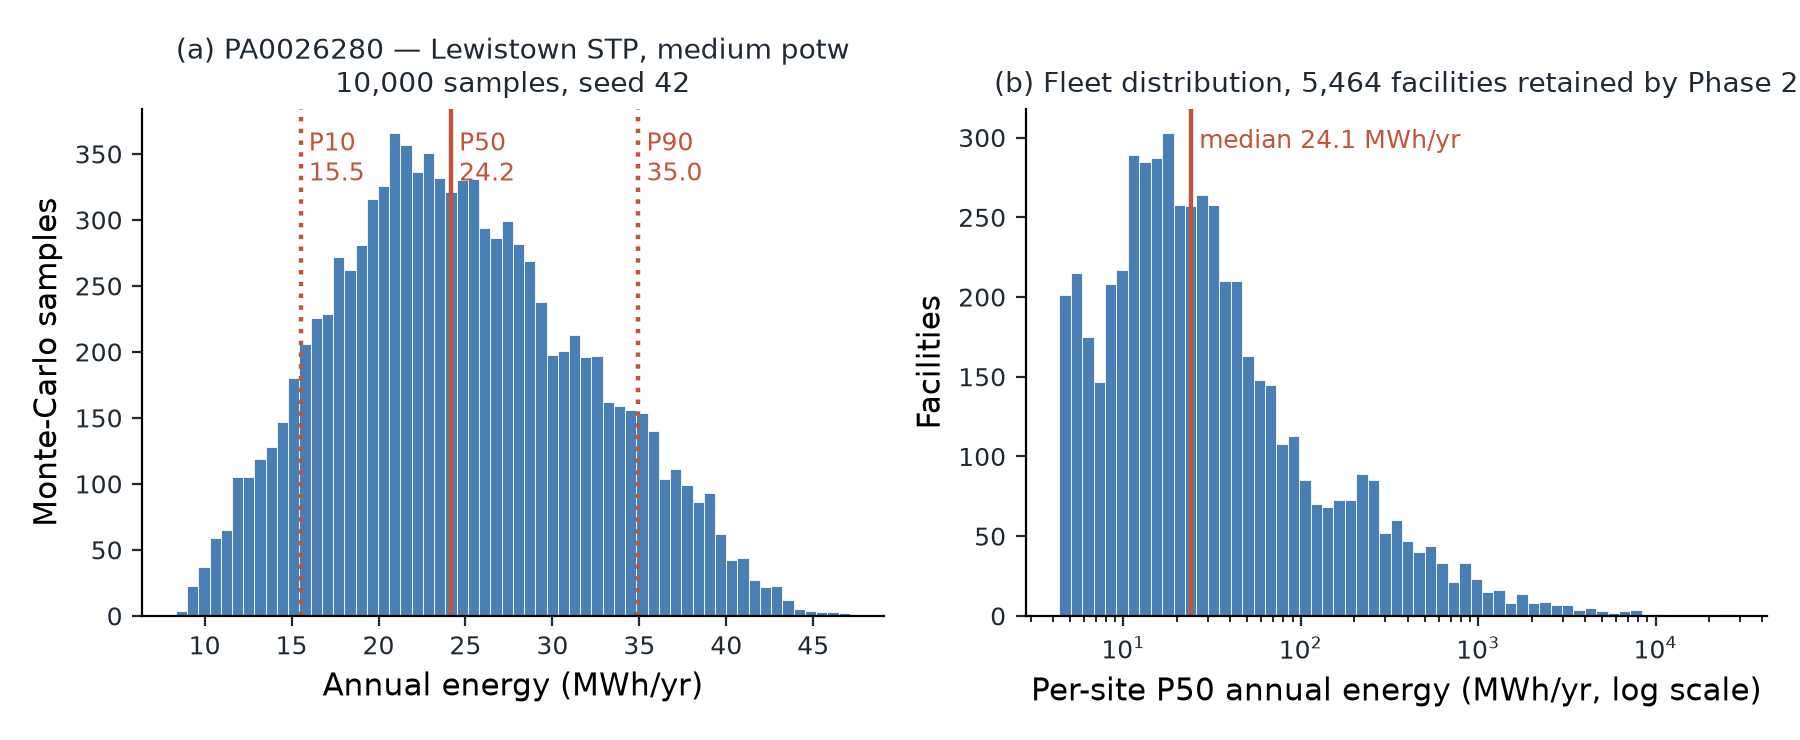
\includegraphics[width=\linewidth]{figures/fig02_mc_energy.png}
\caption{Monte-Carlo annual-energy distribution for a representative plant
(PA0026280, Lewistown STP, 1.59 MGD mean flow, 168 months of DMR record) and the
fleet distribution of per-plant P50 energy for the 5,464 plants retained by
Phase 2}
\label{fig:mc_energy}
\end{figure}

These Phase~2 totals are screening intermediates and are deliberately not the
headline figure of this thesis. They are computed on archetype head rather than
measured head, before turbine sizing, and before economics; the 409.2~GWh/yr
ceiling and the calibrated 119--281~GWh/yr band reported in Chapter~5 come from
Phases~3 and~4 applied to the surviving sites. The gap between 699.18~GWh/yr here
and 409.2~GWh/yr there is a consequence of real head replacing assumed head, of
the 1~kW physics floor, and of the financial gate, and is decomposed stage by
stage in Section~5.1.2.

Four limitations are named. The head triangulars are archetypes indexed by
design flow, not site measurements, and no plant-specific evidence supports the
mode values; Section~4.3.4 replaces them with a digital-elevation-model estimate
and flags that estimate as the largest methodological assumption in the work.
The three sampled quantities are drawn independently, so any real correlation
between head, machine efficiency, and availability is absent from the reported
spread. The FDC integration is truncated to the shorter of the curve and the
exceedance grid, which drops the low-flow tail for plants with sparse records and
understates their annual energy by an estimated few per cent. Finally, the
implied capacity factor is implausibly high: across the 5{,}464 retained plants
its median is 0.869 (tenth to ninetieth percentile 0.834 to 0.883), and across
the 1{,}138 plants that survive to project viability in Phase~4 it is 0.872
(0.856 to 0.883). Part of that is real --- treated wastewater discharge is far
flatter than river flow --- and part is optimism, because a smooth monthly FDC is
integrated as though the machine ran at every point on it with no debris, minimum
flow, or outage modelling. That discrepancy is
not corrected inside Phase~2; it is measured against real capacity factors and
turned into the calibration band in Section~4.4. Head estimation, which removes
the archetype assumption these energy figures rest on, will now be discussed.
\subsection{Head Estimation}
\wptodo{T4 · 4.3.4}{Feeds: head\_estimation.py, outfall\_coords.py. Flag DEM-proxy as the
LARGEST methodological assumption; the plausibility gate.}
\subsection{Turbine Selection}
\wptodo{T4 · 4.3.5}{Feeds: turbine\_selection.py, data/turbines/turbine\_manufacturers.csv.}
\subsection{Cost Models and Financial Scorecard}
\wptodo{T4 · 4.3.6}{Feeds: cost\_models.py, financials.py, revenue.py, plant\_consumption.py,
sensitivity.py, EXCLUSION\_FUNNEL\_REPORT.md. CapEx bands, install cost, NPV/IRR/payback.}

\section{Calibration and Validation}                     % WP T5 — Tom
\wptodo{T5 · 4.4 (~part of 2,000 w)}{Feeds: scripts/cf\_calibration.py,
CF\_CALIBRATION\_REPORT.md, src/phase5/*, FERC\_CONDUIT\_LABEL\_REPORT.md. Implied-CF vs EHA-CF
$\rightarrow$ 119--281 GWh band (strongest element). Phase-5 ML KILL as an honest negative
result — report it, do not hide it.}

\section{Data Export and Serving Layer}                  % WP T5 — Tom
\wptodo{T5 · 4.5}{Feeds: scripts/export\_geojson.py, exports/viable\_sites.geojson +
scored\_sites.geojson. The 58-property contract, byte-determinism.}

\section{Frontend Visualization System}                  % WP M1 — Mohamed [MERGE]
\wptodo{M1 · 4.6 — MERGE FROM MOHAMED (~2,000 w)}{Mohamed drafts in his file; paste here at
combine time. Feeds: frontend/src/ (App routing, 7 views, MapView, charts, Gauge, SiteTable,
lib/data.ts). Stack options; single-file geojson contract; the 7 views; URL filters; CSV;
map interaction.}
% \figplaceholder{2}{Frontend application flow / routing diagram.}{Frontend application flow}

% =====================================================================
% CHAPTER 5 — EXPERIMENTS AND RESULTS (3,500-4,500 w)
% Format quirk: subsections start at 5.1.1; there is NO 5.1 heading.
% =====================================================================
\chapter{Experiments and Results}
% force section counter to 1 (prints no heading) so subsections read 5.1.x
\stepcounter{section}\setcounter{subsection}{0}

\subsection{Best Case and Expected System Performance}   % WP T6 — Tom
\wptodo{T6 · 5.1.1 (must come first)}{Two PARALLEL tables — Ideal vs Expected system
performance — identical columns, differing assumptions. Physics ceiling 409.2 GWh/yr vs
calibrated band 119--281 GWh/yr.}

\subsection{Site Exclusion Funnel}                       % WP T6 — Tom
\wptodo{T6 · 5.1.2}{17,148 $\rightarrow$ 5,464 $\rightarrow$ 4,860 $\rightarrow$ 3,778
$\rightarrow$ 1,138. Selection-bias defense: 76.8\% data-gap vs 16.5\% economics.}
\figplaceholder{8}{Exclusion funnel from 17,148 screened POTWs to 1,138 project-viable
sites, with the drop reason at each stage.}{Site exclusion funnel}

\subsection{Energy and Financial Results}                % WP T6 — Tom
\wptodo{T6 · 5.1.3}{Monte-Carlo energy, portfolio NPV \$310.1M, median payback 9.8 yr.
Discrepancy paragraphs wherever measured $\neq$ expected.}

\subsection{Capacity-Factor Calibration}                 % WP T6 — Tom
\wptodo{T6 · 5.1.4}{Implied-CF vs EHA-CF (629 plants / 9{,}798 plant-years). LucidPipe
Portland CF 0.628 anchor. The calibration-band result + discrepancy paragraph.}

\subsection{Machine-Learning Feasibility (Negative Result)} % WP T6 — Tom
\wptodo{T6 · 5.1.5}{Report the Phase-5 kill plainly: only 11 conduit labels found vs the
$\geq 50$ gate; Point Loma offline since 2018. List the specific reasons it failed.}

\subsection{Frontend Performance}                        % WP M2 — Mohamed [MERGE]
\wptodo{M2 · 5.1.6 — MERGE FROM MOHAMED (~700 w)}{Build perf (vite 7.3.5, ~2.6 s, bundle
sizes), headless + Chrome QA. Separate measured from deferred (code-splitting, clustering).}

\subsection{System Integration Test}                     % WP J4 — Joint
\wptodo{J4 · 5.1.7}{End-to-end: parquets $\rightarrow$ export\_geojson.py $\rightarrow$
dashboard; P2-SEED baseline matches across the boundary (1,138 / 409.17 GWh / \$310.1M /
9.8 yr). Realistic stimulus = the real re-baselined parquets.}

% =====================================================================
% CHAPTER 6 — CONCLUSIONS AND FUTURE WORK               (WP J3 — Joint)
% =====================================================================
\chapter{Conclusions and Future Work}
\wptodo{J3 · Ch6 (~900 w)}{What was designed/tested + which MVP requirements it fulfills;
restate headline metrics at full precision; three future-work themes (Tom-side validation /
head-error; Mohamed-side code-splitting / clustering / live backend; joint customer pilot);
position as first step to customer value.}

% =====================================================================
% REFERENCES  (IEEE-adjacent, numbered by first appearance; target 40-50)
% =====================================================================
\begin{thebibliography}{99}

\bibitem{epri2013}
S.~Pabi, A.~Amarnath, R.~Goldstein, and L.~Reekie,
``Electricity Use and Management in the Municipal Water Supply and Wastewater Industries,''
Electric Power Research Institute, Report 3002001433, Nov.\ 2013.

\bibitem{epa2013}
U.S.\ Environmental Protection Agency,
``Energy Efficiency in Water and Wastewater Facilities,''
Local Government Climate and Energy Strategy Series, EPA 832-R-10-005, 2013.

\bibitem{wef_mop32}
Water Environment Federation,
\emph{Energy Conservation in Water and Wastewater Treatment Facilities},
Manual of Practice No.~32, WEF Press, Alexandria, VA, 2009.

\bibitem{epa_echo}
U.S.\ Environmental Protection Agency,
``Enforcement and Compliance History Online (ECHO) / ICIS-NPDES Data Downloads,''
[Online]. Available: https://echo.epa.gov/

\bibitem{usgs_3dep}
U.S.\ Geological Survey,
``3D Elevation Program (3DEP),''
[Online]. Available: https://www.usgs.gov/3d-elevation-program

\bibitem{hydrosource_eha}
Oak Ridge National Laboratory,
``Existing Hydropower Assets (EHA) --- Annual Capacity Factor,''
DOE HydroSource, [Online]. Available: https://hydrosource.ornl.gov/

\bibitem{doe_vision}
U.S.\ Department of Energy,
\emph{Hydropower Vision: A New Chapter for America's 1st Renewable Electricity Source},
DOE/EE-1504, 2016.

\bibitem{ornl2014}
S.-C.~Kao et al.,
``New Stream-reach Development: A Comprehensive Assessment of Power Energy Potential on Existing Streams within the United States,''
Oak Ridge National Laboratory, ORNL/TM-2014/525, 2014.

\bibitem{osti3002705}
Oak Ridge National Laboratory,
``Municipal Conduit Hydropower Project Cost Data,''
OSTI 3002705 (supporting tables), ca.\ 2020\$ basis.

\bibitem{lucidpipe}
LucidEnergy / Portland Water Bureau,
``LucidPipe Power System --- Portland, Oregon (Bull Run transmission main),''
project documentation and press materials; see also technical overview at thecivilengineer.org.

\bibitem{rentricity}
Rentricity Inc.,
``Featured Projects,''
[Online]. Available: https://rentricity.com/featured-projects

\bibitem{cink}
CINK Hydro-Energy,
``References and Wastewater Applications,''
[Online]. Available: https://cink-hydro-energy.com/references

\bibitem{ferc_conduit}
Federal Energy Regulatory Commission,
``Qualifying Conduit Hydropower Facilities,''
18~CFR~4.400--4.401; Hydropower Regulatory Efficiency Act of 2013.

\bibitem{eia_household}
U.S.\ Energy Information Administration,
``How much electricity does an American home use?,'' Frequently Asked Questions,
2023 residential average (10,500~kWh/yr per customer).
[Online]. Available: https://www.eia.gov/tools/faqs/faq.php?id=97
% Additional Track M / Joint citations merge here at WP J5.

\end{thebibliography}

% =====================================================================
% APPENDICES                                            (WP T7 — Tom)
% =====================================================================
\appendix
\chapter{Data Dictionary and Exclusion-Funnel Tables}
\wptodo{T7 · Appendix A}{58 geojson properties; full funnel tables.}
\chapter{Calibration and Sensitivity Captures}
\wptodo{T7 · Appendix B}{Implied-CF vs EHA-CF captures; sensitivity NPV bands.}
\chapter{Monte-Carlo Distribution Figures}
\wptodo{T7 · Appendix C}{P10/P50/P90 distributions.}

\end{document}
